Rosesland cuenta con dispositivos tipo tablet, por lo que el diseño de la interfaz de usuario debe aprovechar las ventajas que ofrece este entorno interactivo. Se pretende resumir el proceso de venta, elaboracion y entrega de productos en dos secciones. También se agrega una sección de administración de usuarios y una página con información general de las florería.
\vspace{0.8cm}

\begin{figure}[H]
  \centering
  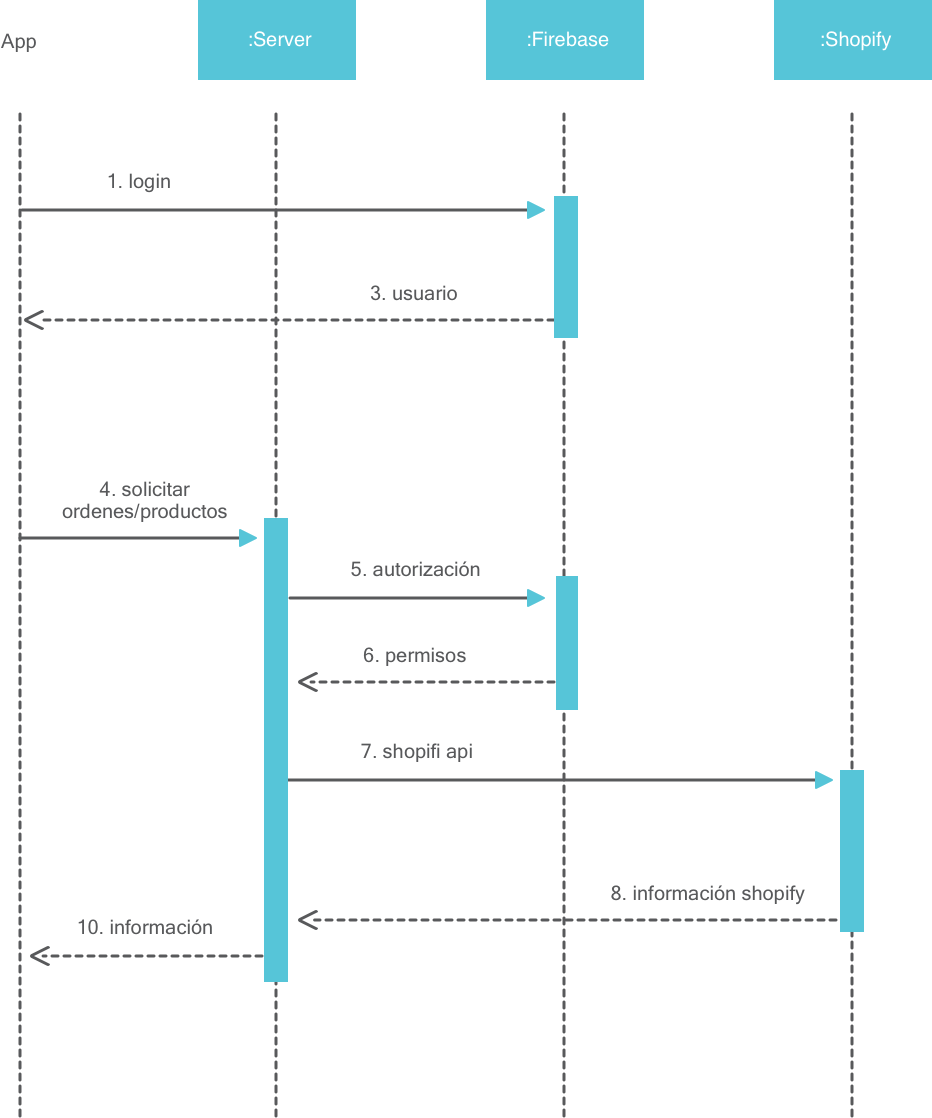
\includegraphics[width=0.75\textwidth]{secuence}
  \caption{Diagrama de secuencia del proceso de autorización.}
\end{figure}
\vspace{0.8cm}

\begin{figure}[H]
  \centering
  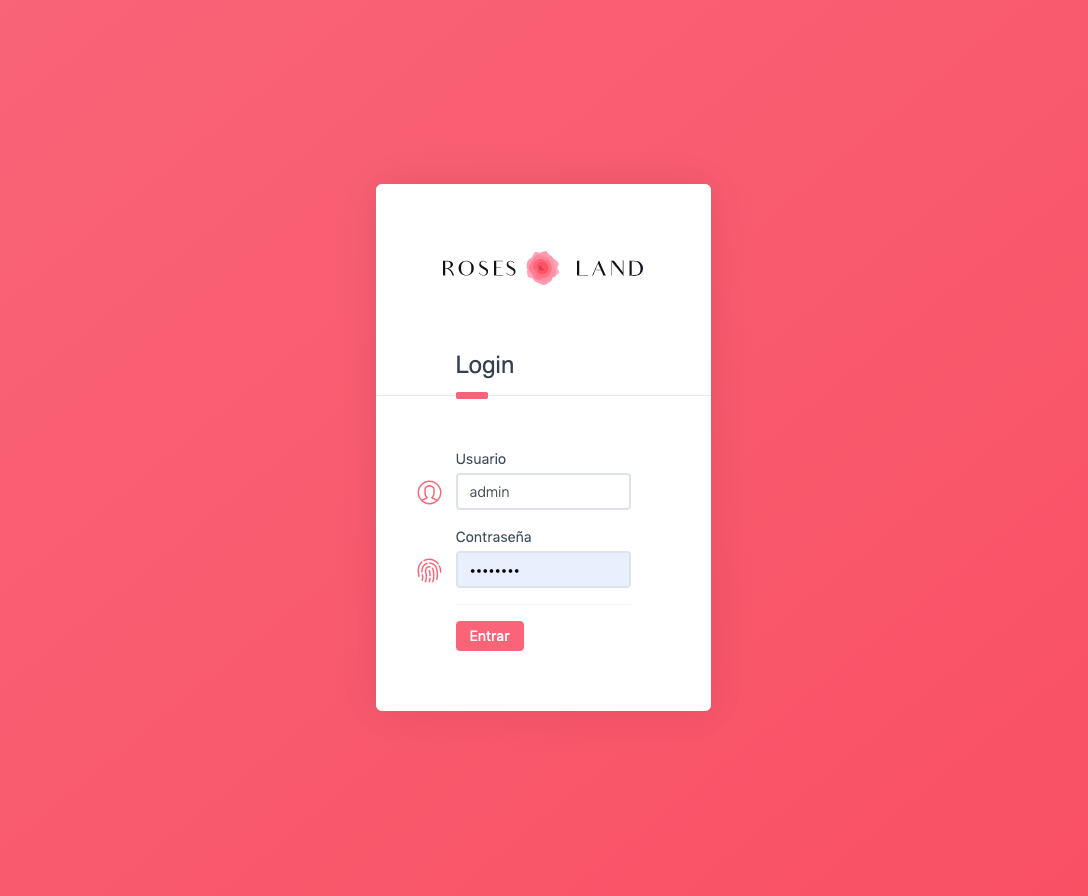
\includegraphics[width=1\textwidth]{app-login}
  \caption{Módulo de inicio de sesión.}
\end{figure}
\vspace{0.8cm}

\begin{figure}[H]
  \centering
  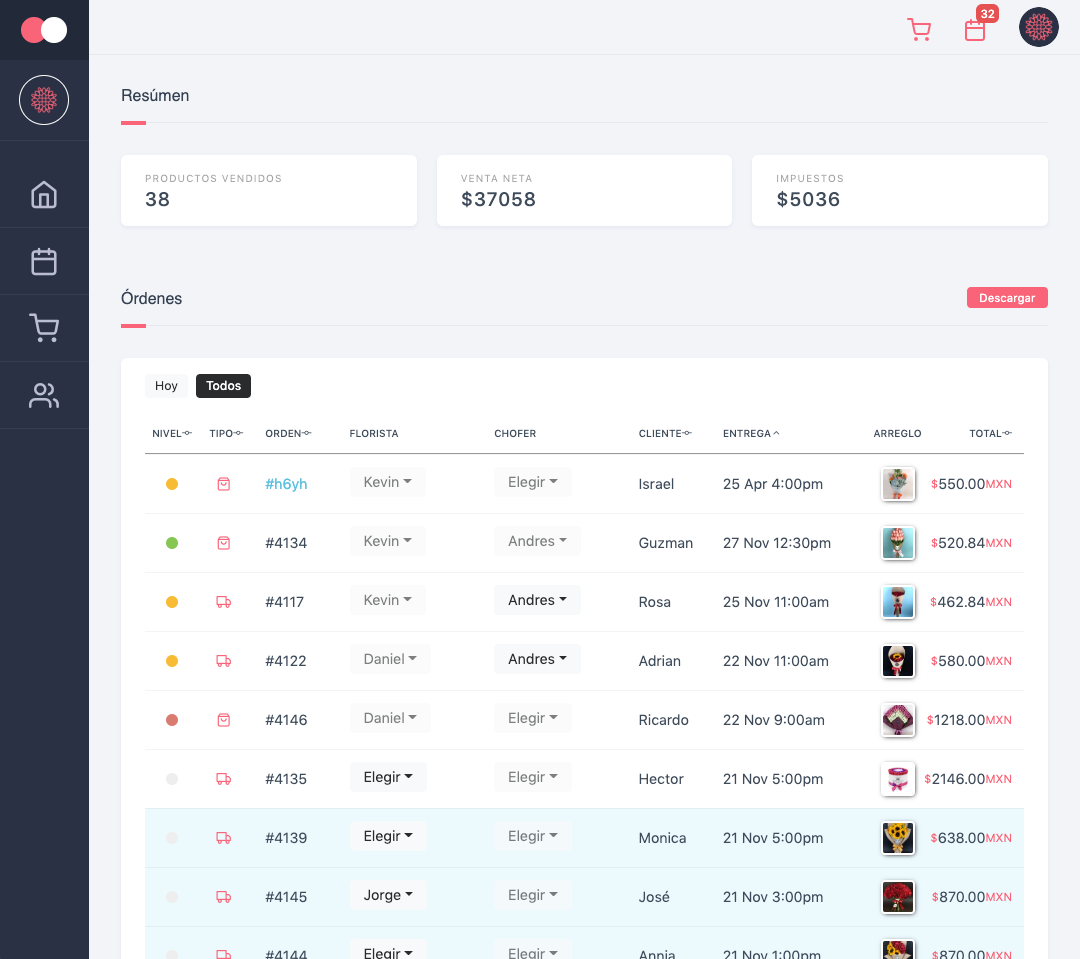
\includegraphics[width=1\textwidth]{app-main}
  \caption{Sección principal.}
\end{figure}
\vspace{0.8cm}

\begin{figure}[H]
  \centering
  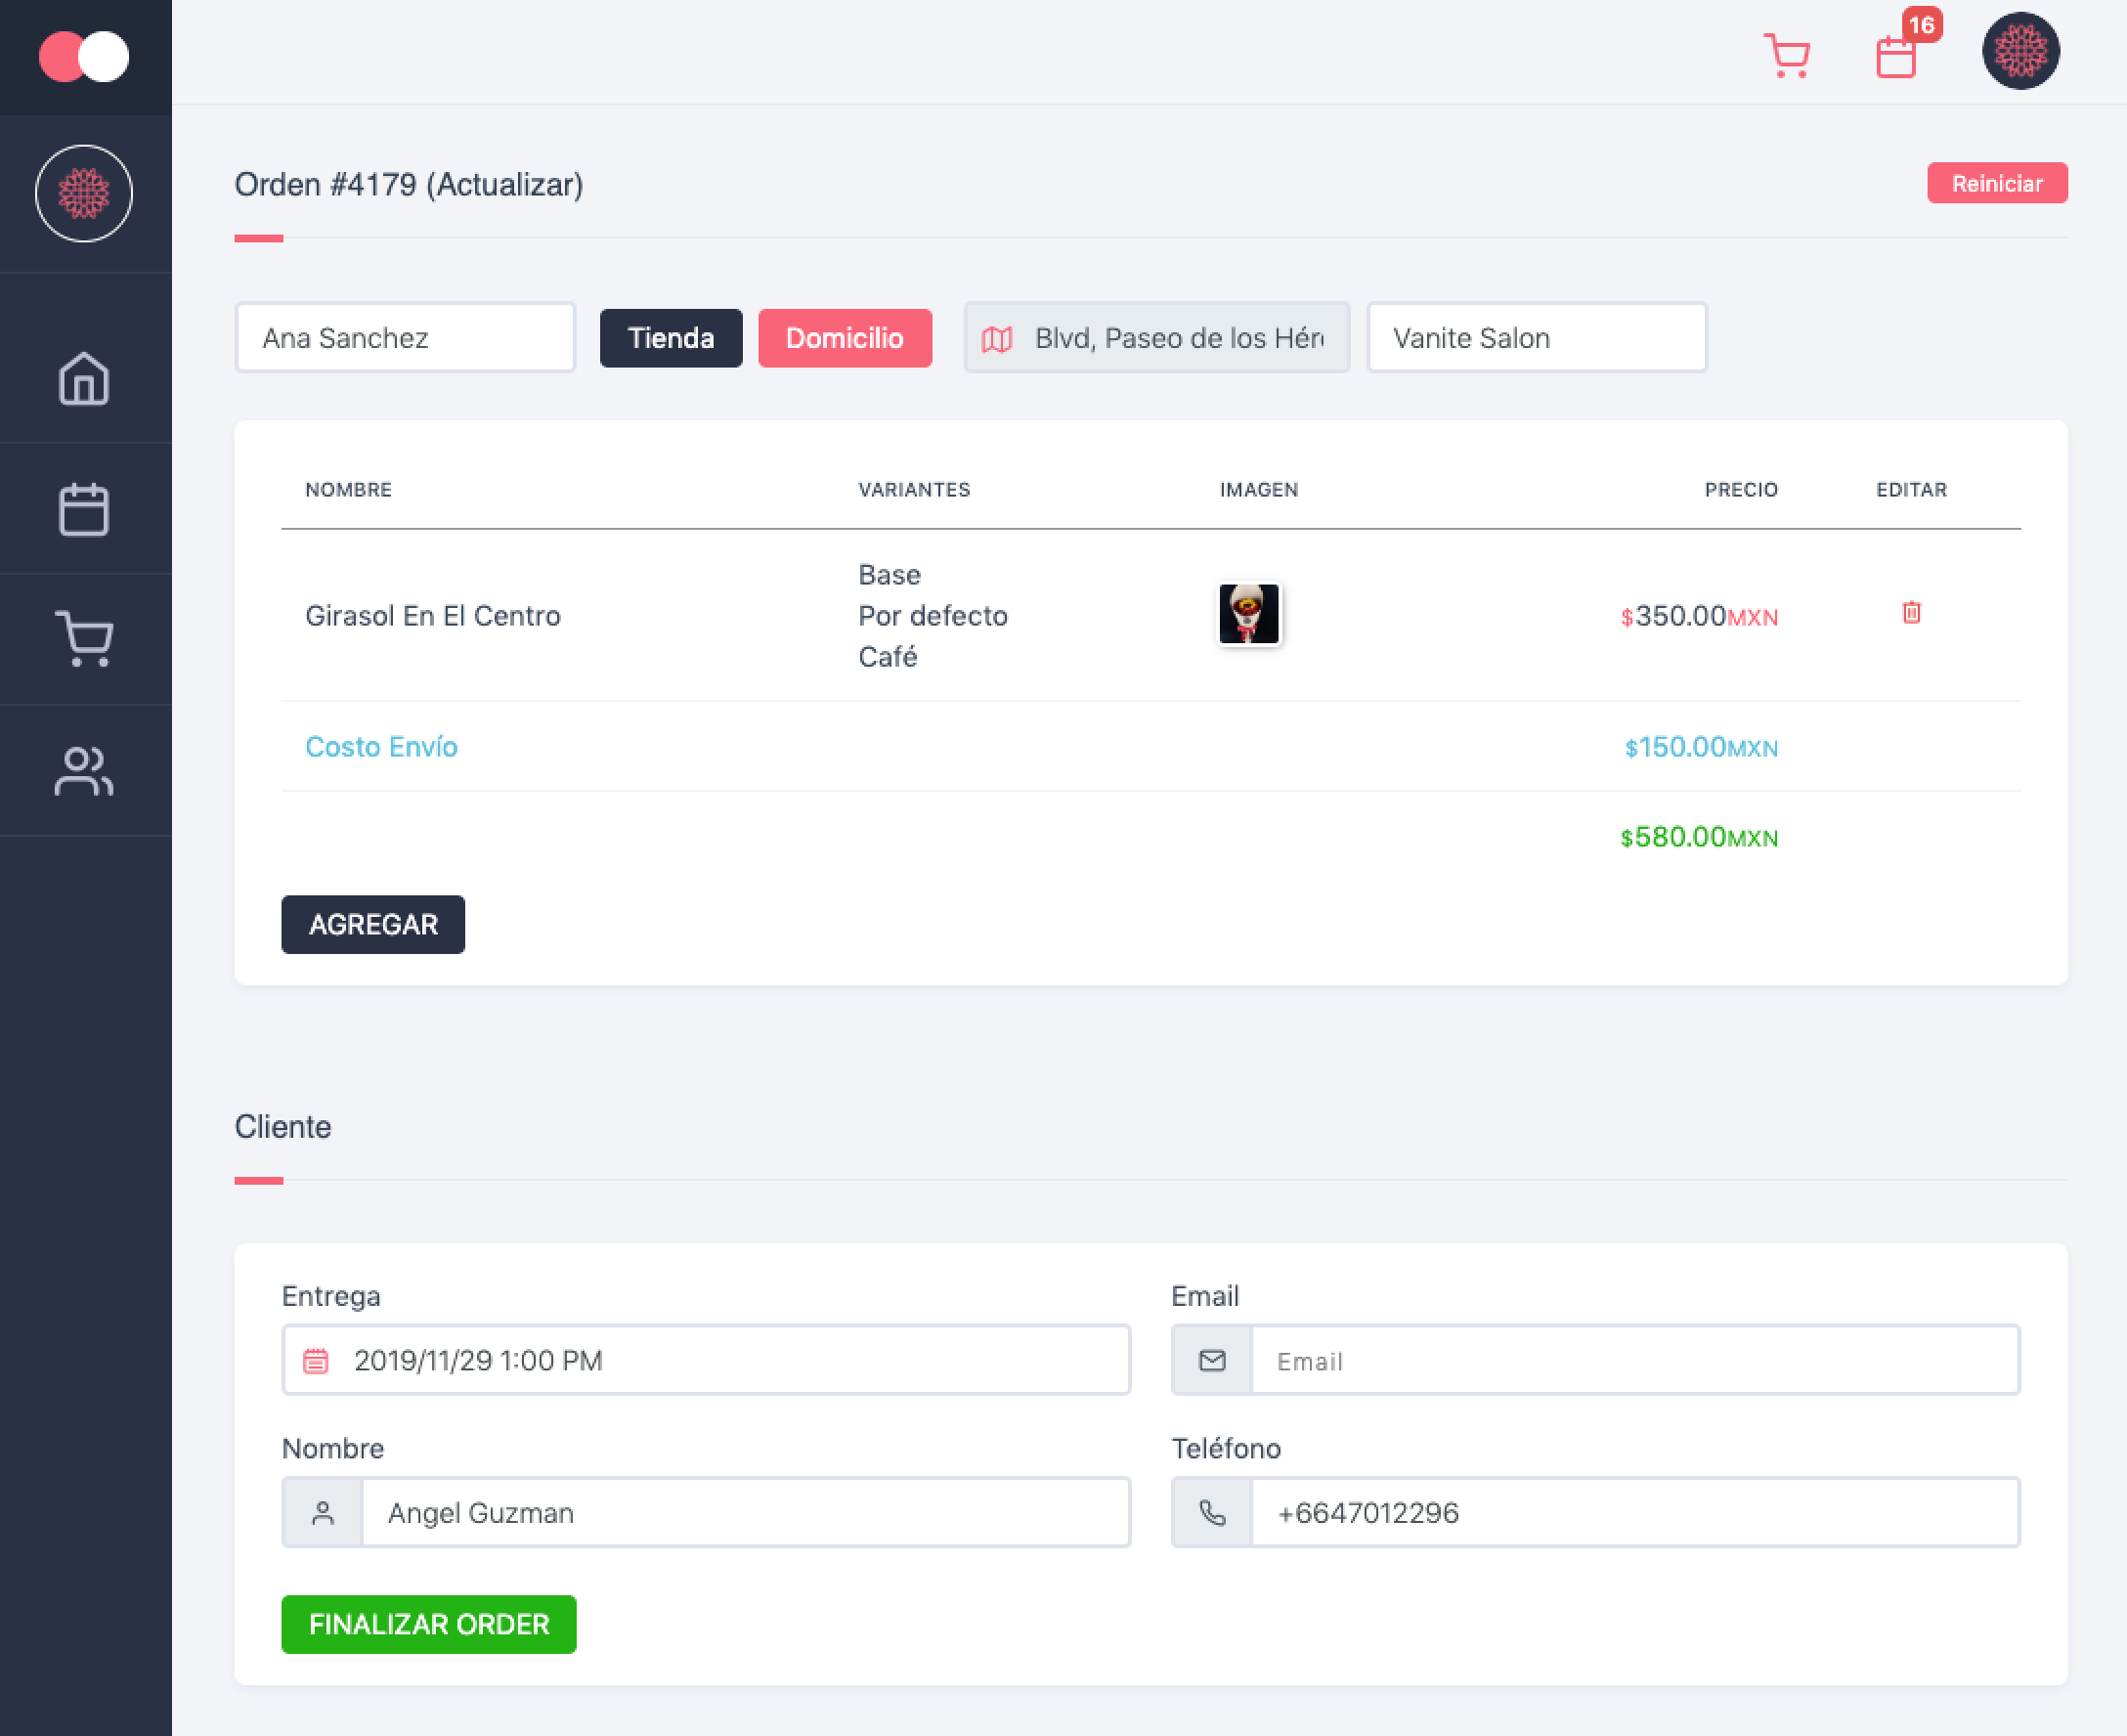
\includegraphics[width=1\textwidth]{app-sales}
  \caption{Sección de ventas.}
\end{figure}
\vspace{0.8cm}

\begin{figure}[H]
  \centering
  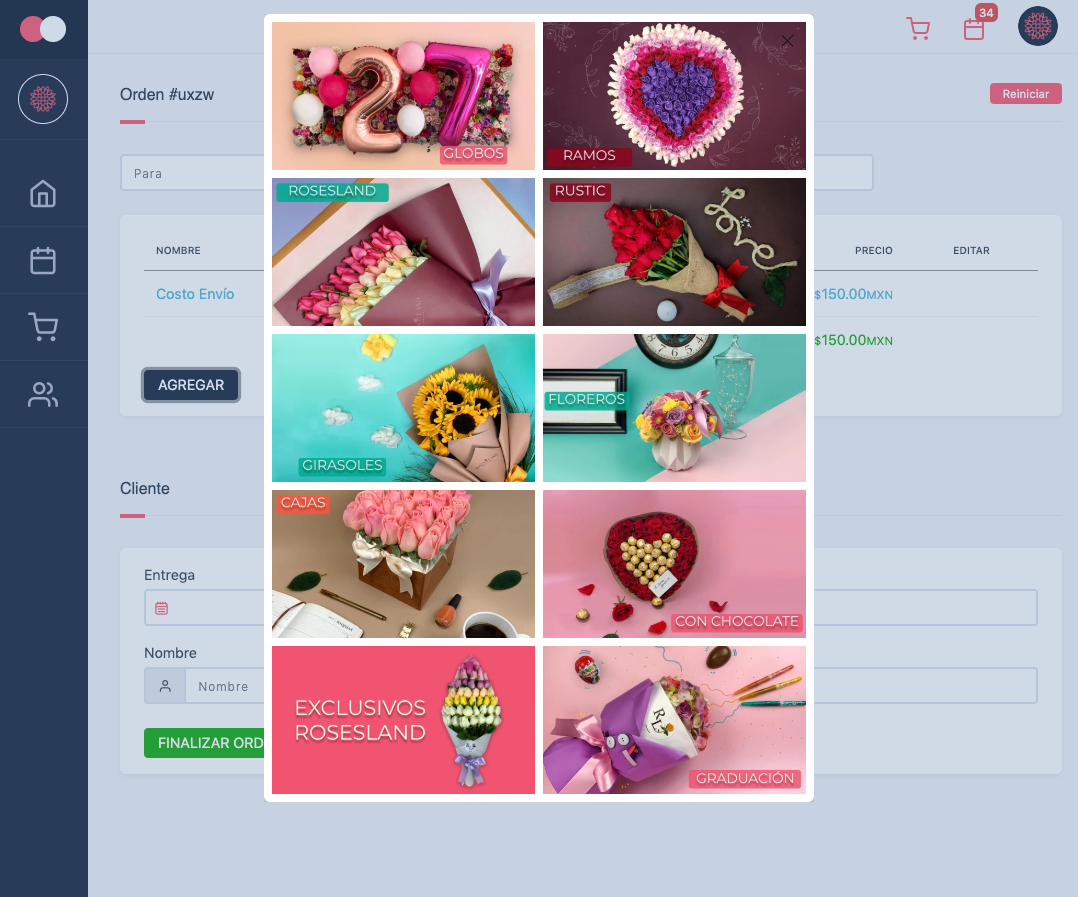
\includegraphics[width=1\textwidth]{app-catalog}
  \caption{Módulo de catálogo de productos.}
\end{figure}
\vspace{0.8cm}

\begin{figure}[H]
  \centering
  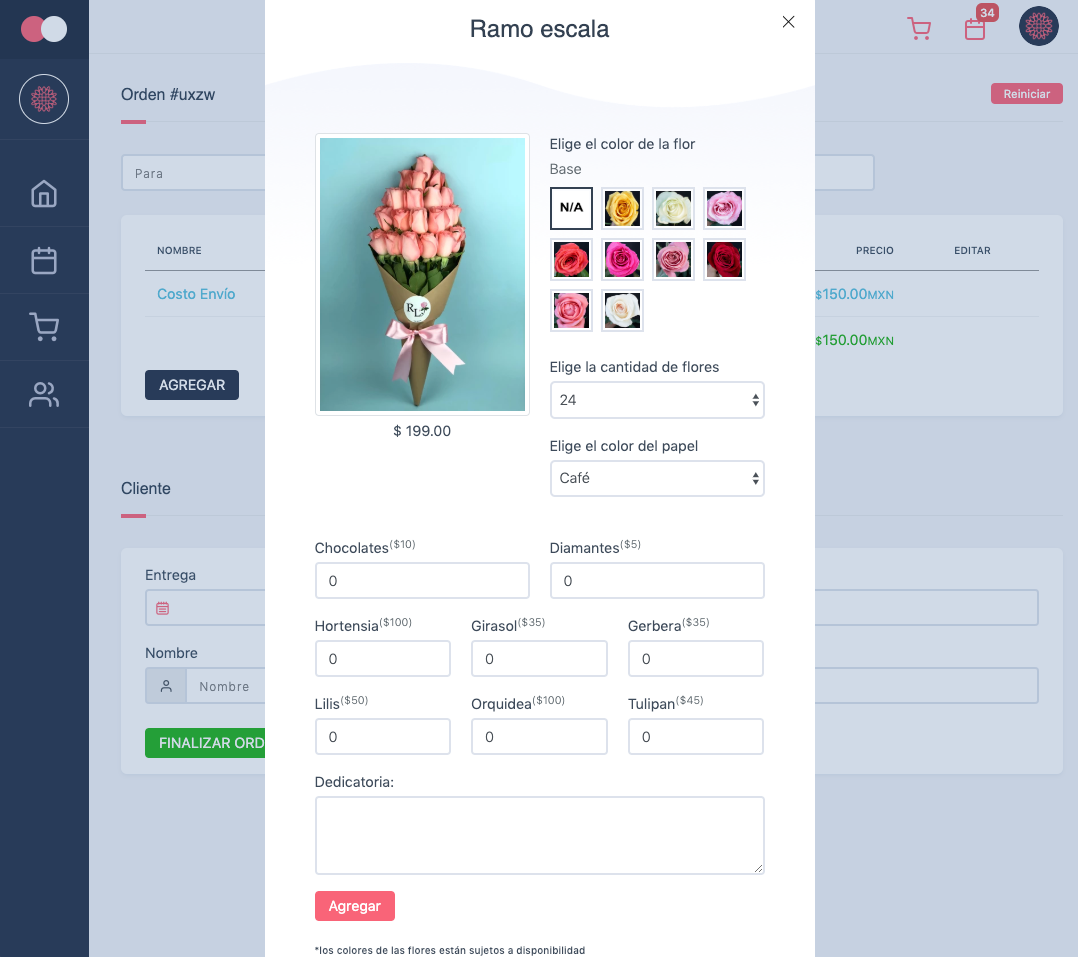
\includegraphics[width=1\textwidth]{app-single}
  \caption{Módulo de producto.}
\end{figure}
\vspace{0.8cm}k

\begin{figure}[H]
  \centering
  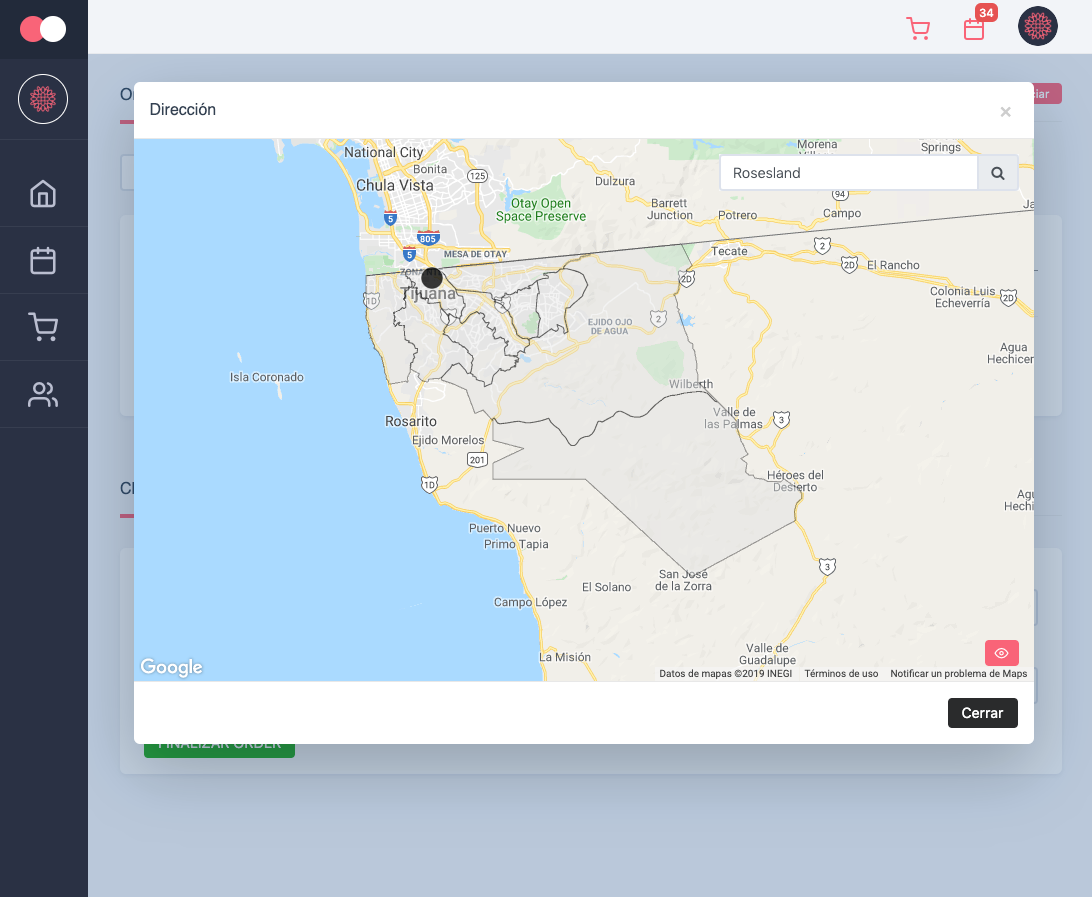
\includegraphics[width=1\textwidth]{app-map}
  \caption{Módulo de Google Map.}
\end{figure}
\vspace{0.8cm}

\begin{figure}[H]
  \centering
  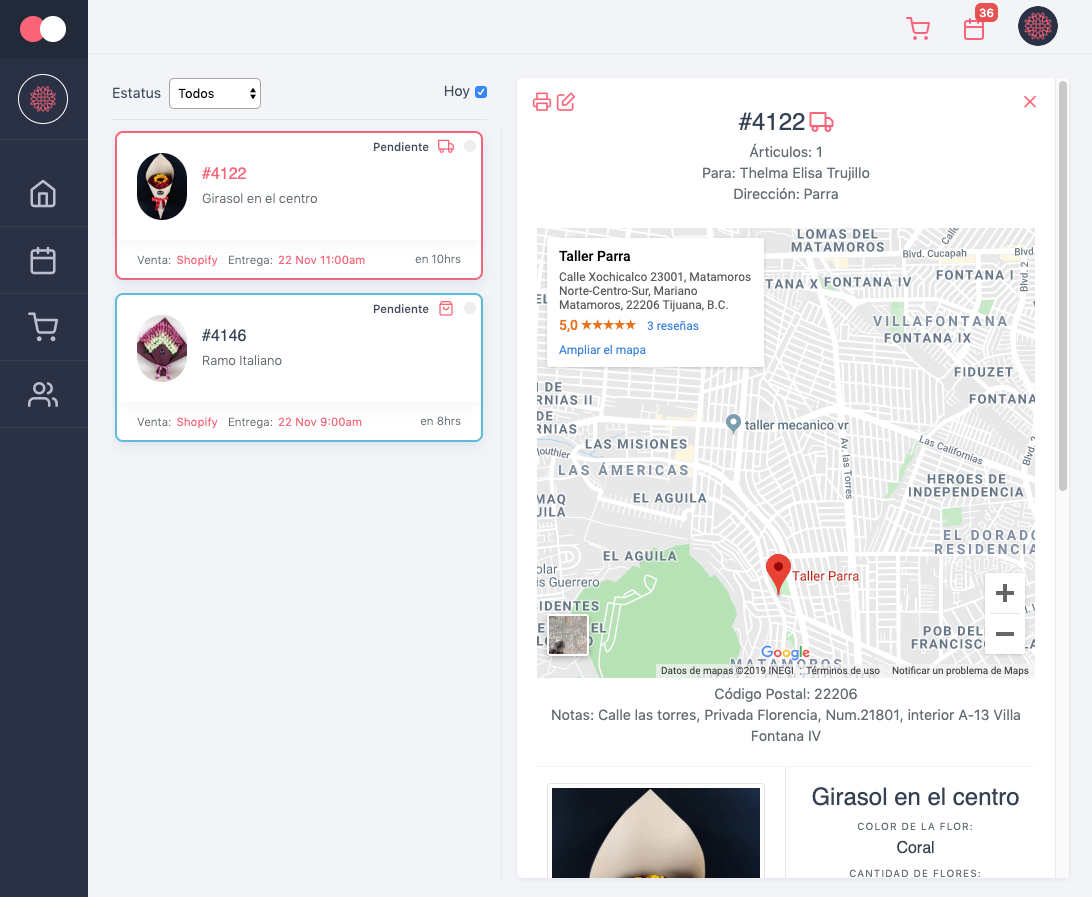
\includegraphics[width=1\textwidth]{app-orders}
  \caption{Módulo de manufactura y entrega.}
\end{figure}
\vspace{0.8cm}

\begin{figure}[H]
  \centering
  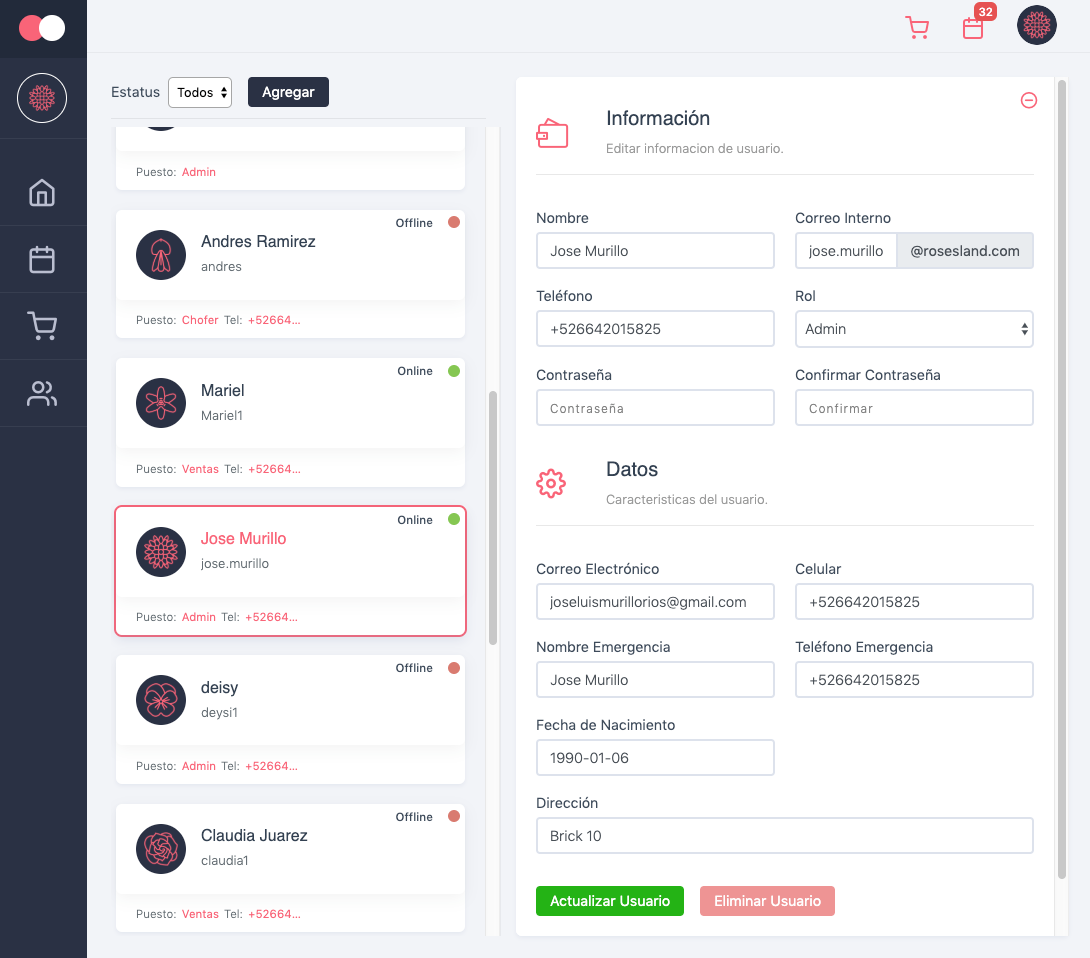
\includegraphics[width=1\textwidth]{app-admin}
  \caption{Módulo de administración de usuarios.}
\end{figure}
\vspace{0.8cm}

\begin{figure}[H]
  \centering
  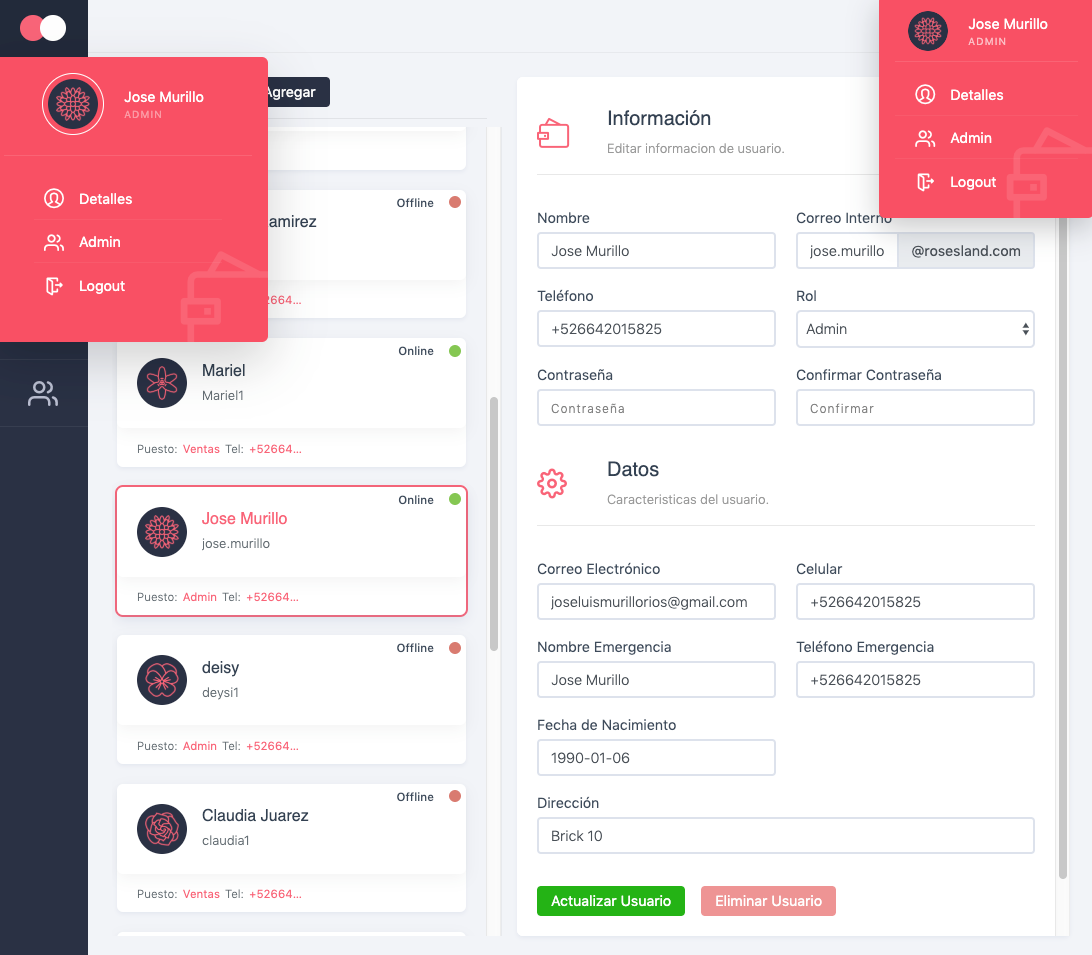
\includegraphics[width=1\textwidth]{app-atomic}
  \caption{Implementación Redux y Diseño Atómico.}
\end{figure}
\vspace{0.8cm}